
\chapter{Extending and Enhancing Sampling-based PBM}
\label{ch:extending-sampling}
This chapter describes improvements to PBM-sampling, some of which are general improvements for all workloads and others allow PBM-sampling to perform well on workload types beyond what PBM-PQ specialises in.

\section{Bulk Eviction\label{sec:sampling-bulk-eviction}}

PBM-PQ evicts several pages at once to amortize the CPU cost of eviction.~\cite{pbm} With sampling, there is not a direct CPU benefit to evicting multiple blocks at once, but better hit rate is achievable for the same CPU cost with a similar bulk eviction technique.

Rather than choosing $N$ buffers from the cache and evicting only one each time a buffer is allocated, consider taking a sample of $kN$ buffers and evicting the $k$ buffers from the sample with largest next-access time. This technique considers the same $kN$ buffers over a sequence of $k$ buffer allocations, but can make better eviction decisions by considering them all together rather than separately.

With separate single evictions, it is possible that one sample may not contain any good candidates resulting in a bad eviction, while another sample may contain multiple good eviction candidates but will select only one. With bulk eviction, it is as if one can take a surplus good eviction candidate from a different recent or near-future sample instead of evicting the bad candidate, thus reducing the over-all rate of bad eviction choices. Using the example in Figure \ref{fig:multi-eviction}, the first eviction samples two good eviction candidates while the second eviction samples only items that should be kept in the cache, so with single eviction it would end up making a bad eviction. Using bulk eviction for this scenario, the same sampled cache items from multiple consecutive evictions are considered together allowing both good candidates from the first single-eviction sample to be evicted and avoiding evicting something which would optimally be kept in the cache. Appendix~\ref{sec:sampling-probabilities} analyses and demonstrates this benefit mathematically.


\begin{figure}
    \centering
    \begin{subfigure}{\columnwidth}
        \centering
        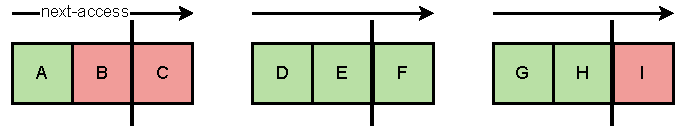
\includegraphics[width=\columnwidth]{figures/Diagrams/diagrams-multi-eviction-a.pdf}
        \caption{Multiple single evictions each evict the single item with latest next-access from a limited sample.}
    \end{subfigure}
    \vspace{5pt}
    \begin{subfigure}{\columnwidth}
        \centering
        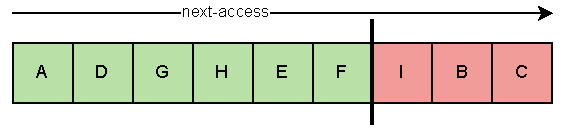
\includegraphics[width=0.8181818\columnwidth]{figures/Diagrams/diagrams-multi-eviction-b.pdf}
        \caption{Bulk-eviction considers the same samples, with a better set of eviction choices.}
    \end{subfigure}
    
    \caption[Bulk eviction example]{Bulk eviction example with $N=k=3$. The colour identifies MIN-optimal eviction candidates as in Figure~\ref{fig:belady-boundary}, and items to the right of the vertical bars are chosen for replacement.}
    \label{fig:multi-eviction}
\end{figure}

With this technique the total number of samples chosen -- and therefore next-access estimates computed -- stays the same compared to single-eviction, so the CPU cost is practically the same, but the eviction decisions are better so hit rate is improved.


% With more evictions together there is a larger gap between when eviction decisions are made and when the block is actually replaced in the cache. With too many evictions at once this gap means evictions decisions are effectively made earlier than the actual eviction, running the risk of bad eviction decisions based on old data, but for a small number of evictions at once the time to replace all blocks chosen for eviction is very small.



\section{\label{sec:frequency-stats}Frequency Statistics}

\citet{pbm} mention, but do not implement, an extension to PBM-PQ using frequency statistics to prioritize cache blocks that are not requested by any active sequential scans. This is not expected to help for workloads with only long-running sequential scans, but could be useful for smaller tables and index lookups. The method proposed by \citet{pbm} is to store a few recent access times for each block, and store non-requested blocks in a separate set of buckets corresponding to the inter-access time. The second set of buckets ages over time, equivalently increasing the estimated time-to-next-access of these blocks.

This thesis pursues this proposal by developing a similar idea to track frequency statistics in PBM-sampling that is much easier to implement as discussed in Chapter~\ref{sec:sampling-advantages}. In PBM-sampling, the system tracks an exponentially weighted moving average of the time between accesses (inter-access time) for each block in the cache. With sampling no special data structures are needed to handle this scenario, just some extra fields in the existing buffer headers. As depicted in \Cref{alg:sampling_freq}, if the time-since-last-access is less than the average inter-access time, the frequency-based time-to-next-access is estimated to be the average inter-access time. Once the time-since-last-access exceeds the average inter-access time, the time-since-last-access is used as the estimated time-to-next-access instead to decrease the relative priority of these blocks over time. 

\begin{algorithm}[]
\SetAlgoLined
\SetNoFillComment
\DontPrintSemicolon
\SetKw{KwReturn}{return}
\SetKwFunction{FFreqNextAccess}{EstNextAccessFreq}
\SetKwProg{Fn}{Function}{:}{}

\Fn{\FFreqNextAccess{blk}}{
    t\_since\_access $\gets \text{now} - \text{blk.last\_access}$\;
    \uIf{blk.num\_access $\le 1$}{
        % \tcc{fall-back to LRU}
        \tcc{not enough recent access information}
        \KwReturn $\infty$\;
    }\uElseIf{$\text{blk}.\text{avg\_inter\_access} < \text{t\_since\_access}$}{
        \KwReturn blk.avg\_inter\_access\;
    }\Else{
        \KwReturn t\_since\_access\;
    }
}\;

\caption{Next-access-time estimate based on recent inter-access times.}
\label{alg:sampling_freq}

\end{algorithm}

If a block is also registered by a sequential scan, the resulting next-access estimate is the minimum of the frequency-based and registered-scan-based estimates.

These stats are only kept for blocks currently in the cache, so newly loaded blocks will not have an inter-access time since they have been accessed only once. Newly loaded blocks are therefore more likely to be evicted prematurely if they are not also requested by a sequential scan. This is mitigated with sampling since, on average, some time will pass before the blocks will be sampled. The next sub-chapter discusses another method for handling the case of non-requested blocks.

\section{\label{sec:lru_nr}Fallback to LRU}


The original implementation of PBM-PQ \cite{pbm} uses \gls{lru} to prioritize amongst blocks that are not requested sequentially.\footnote{The PostgreSQL implementation of PBM-PQ in this thesis takes a different approach, discussed in Chapter~\ref{sec:pbm-pq_postgres}.} With the sampling-based strategy, the frequency statistics described in Chapter~\ref{sec:frequency-stats} mostly serves the same purpose, but as mentioned it has a blind-spot for blocks that are new to the cache and have not yet been accessed multiple times. A technique that can be used to improve this case is to use \gls{lru} as a tie-breaker for blocks that are not requested sequentially and do not have frequency statistics. If multiple sampled blocks are not requested sequentially and do not have frequency statistics, the system will prefer to keep the ones that have been accessed more recently and evict the one accessed least-recently. % or, if freqency stats are disabled it can use this instead


\section{\label{sec:index_scans}Index scans}

So far the discussion has been mainly about sequential access patterns. Sequential scans are the most efficient way to read a large data-set when most of the data is needed to answer a query, but secondary indexes can greatly reduce I/O and CPU cost for workloads where this is not the case. PostgreSQL supports various types of indexes, so they should also be considered to inform caching decisions.

Unfortunately, index scans do not generally have a predictable order for accessing secondary storage, so they are not as easy to predict as sequential scans. There are, however, a few situations where the information from an index scan may be useful to help make eviction decisions.

\subsection{\label{sec:bitmap_scans}Bitmap index scans}

In PostgreSQL, any index can be scanned as a bitmap scan. In this case, the system first reads only the index and constructs a bitmap indicating which tuples might match the query predicate. The table is then scanned in sequential order, using the bitmap to skip blocks that do not contain any matching tuples. Bitmap scans can be selected by the query planner for any type of index, but certain index types can only be used with bitmap scans. Most notably, PostgreSQL's block range indexes (BRIN) always use bitmap scans. BRIN splits the table into ranges of blocks and stores a summary of each range, which can be compared to the query predicate to quickly rule out all tuples from a range. The default form of BRIN is a min-max index, where the summaries store the column's minimum and maximum value for each range of blocks, and it also supports bloom filter summaries and a few other strategies for specific data types.

Bitmap scans are the best-case for index scans with predictive buffer management: the order is predictable and the set of blocks to be retrieved is known early, after constructing the bitmap. It is easy to support bitmap scans in both sampling-based and priority-queue based \gls{pbm} as the only necessary change is to how the scan is initially registered. The \gls{pbm} registration happens after the scan operator constructs the bitmap, and the bitmap itself is used to determine which blocks will be scanned and when, but the rest of the implementation is the same as for sequential scans. This is depicted in \Cref{fig:bitmap_scan_tracking}.

The original implementation of PBM-PQ supports automatically created min-max indexes in a similar way~\cite{pbm}, but PostgreSQL's bitmap scans are more general and apply to more types of indexes.

\begin{figure}
    \centering
    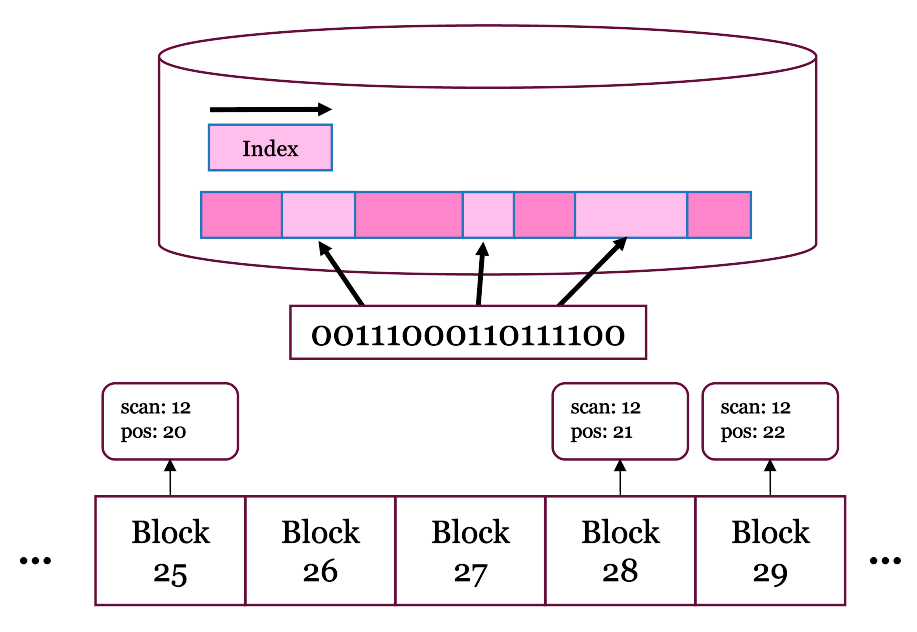
\includegraphics[width=1\columnwidth]{figures/Diagrams/bitmap_scan_registered_progress.png}
    \caption[PBM bitmap scan tracking]{Bitmap scans are handled similar to sequential scans in \Cref{fig:scan_tracking}. After the bitmap is constructed from the index, the bitmap is used to register only blocks relevant to the scan. Time-to-next-access is estimated for each block in the same way as with sequential scans.}
    \label{fig:bitmap_scan_tracking}
\end{figure}

\subsection{Trailing index scans}
\label{sec:idx_trailing}

Certain index types -- such as B-tree indexes -- return their results in sorted order. Thus two independent index range scans with overlapping ranges will visit the tuples from the shared part of the range in the same order. When there are concurrent index range scans on the same relation, the system can detect the shared scan range and use information from one scan to know what the next scan will access.

The way a trailing index scan is detected involves marking blocks as they are accessed by the leading scan for the trailing scan to detect when it reaches the same point. When an index scan accesses a block it records in the buffer header: the current time, which tuple from the block was accessed, and which index is used. When another index scan reaches the same tuple, it checks the mark to determine whether it is following another scan. If the mark is for the same index and the same tuple, the scan knows it is trailing the scan that left the mark and can calculate how far behind it is based on the recorded timestamp. It then notifies the leading scan that it is trailing with a certain delay, and the leading scan will also start marking blocks it accesses with the time it estimates the trailing scan will also reach that block. Estimating next-access-times will now use the estimate left by the leading scan if this estimate is less than the access time suggested by other factors.

% ... Alternate (unimplemented) idea for detecting trailing scan: Modify the B-Tree structure to know the current position w.r.t. the index order. Can do this by modifying the internal nodes to store the size (\# of leaves) in each subtree. When searching the tree for the starting point of the range, add up the number of leaves in the subtrees left of the search path to know the position of the first tuple in the index order. Then multiple scans can be ordered by their position to determine how many tuples apart they are in the index order.


\subsection{Almost-sequential index scans}
\label{sec:idx_seq}

Some columns in a table are highly correlated with the physical order of the table. Such columns are good candidate for BRIN indexes, but a B-Tree index can make sense when the query optimizer also wants to sort by that column efficiently. Due to the correlation between the column order and physical order, even an index scan on the column will access the disk blocks in a mostly-sequential order. The PostgreSQL optimizer already has statistics for how correlated an index scan will be with the physical order, so when the correlation is high the index scan can be treated more like a sequential scan. Then the system can estimate when a specific scan will reach a specific block based on the scan's current position and distance between the current and target block, and how fast the scan is progressing.

% Why this might not work well:
%  - for the microbenchmark I came up with, the scan jumps backwards 4k blocks from one key to the next (I only looked at a tiny part of the data, maybe worse over-all). 
%  - so at any time, there is ~320 MiB that could be accessed in the very-near future, which is too much to reasonably keep cached per query.


% \textbf{Inverse frequency}: ...

\subsection{Random access}

For less predictable accesses, such as point look-ups or index scans with no correlation between index and physical order, it is much more difficult to reliably estimate next-access-times. In these scenarios, the frequency statistics from Chapter~\ref{sec:frequency-stats} are a reasonable heuristic for detecting hot-spots in the data.
